\chapter{Basics}
\label{Basics}

\section{Notational Conventions}
\label{Basics:Notation}

Every point $\V{\xi} \in \R^3 \setminus \set{\V{0}}$ given in Cartesian coordinates by the vector 
$\paren{x_1,x_2,x_3}^{\transp}$ can be uniquely described in spherical coordinates by a vector
$\paren{r,\vtheta,\vphi}^{\transp}$ with $r \in \Rp$, $\vtheta \in \interv{[}{0}{\pi}{]}$ and 
$\vphi \in \interv{[}{0}{2\pi}{)}$.
It holds 
\begin{eqnarray*}
  \paren{x_1,x_2,x_3}^{\transp} & = & \paren{r \sin \vtheta \cos \vphi, r \sin \vtheta \sin \vphi, r \cos \vtheta}^{\transp}\\
  r & = & \sqrt{x_1^2+x_2^2+x_3^2} = \norm{\V{\xi}}_2.
\end{eqnarray*} 
We denote by $\twosphere$ the $2$-nd unit sphere embedded into $\R^3$, i.e. 
$$\twosphere := \pset{\V{\xi} \in \R^{3}}{|}{\norm{\V{\xi}}_2=1}$$ 
and identify $\V{\xi} \in \twosphere$ with the vector $\paren{\vtheta,\vphi}^{\transp}$. The 
spherical coordinate system is illustrated in Figure \ref{sphere}.

Now let $\V{\xi} = \paren{\vtheta,\vphi}^{\transp}$, $\V{\eta} = \paren{\vtheta',\vphi'}^{\transp} \in
\twosphere$ and $\alpha$ be the angle spanned by the origin, $\V{\xi}$ and $\V{\eta}$.
Then the standard scalar product
$\scalarproduct{\V{\xi}}{\V{\eta}}_{2} = \cos\left(\alpha\right)$ is given by
\begin{equation}
  \nonumber
  \fun{\cos}{\alpha} = \cos\vtheta\cos\vtheta' +
  \sin\vtheta\sin\vtheta'\fun{\cos}{\vphi-\vphi'}.
\end{equation}

The space of \emph{homogeneous polynomials} of degree $n \in \NZ$ in $\R^3$ is denoted by
$\fun{\text{Hom}_n}{\R^3}$, comprising all polynomials $Q_n \in \Pol_{n}\paren{\R}$ fulfilling 
$\fun{Q_n}{\alpha\:\V{\xi}} = \alpha^n \fun{Q_n}{\V{\xi}}$ for arbitrary $\alpha \in \R$ and $\V{\xi}
\in \R^3$. The proper subspace of \emph{harmonic homogeneous polynomials} of
degree $n$ is defined by
\begin{equation}
  \nonumber
  \fun{\text{Harm}_n}{\R^3} = \pset{Q_n \in \fun{\text{Hom}_n}{\R^3}}{|}{\Delta_x Q \equiv 0},
\end{equation}
where $\Delta_x$ is the Laplace-operator
\begin{equation}
  \nonumber
  \Delta_x = \frac{\partial^2}{\partial x_1^2} + \frac{\partial^2}{\partial x_2^2} +
  \frac{\partial^2}{\partial x_3^2}.
\end{equation}
Furthermore, the relations
\begin{equation}
  \fun{\dim}{\fun{\text{Hom}_n}{\R^3}} = \frac{(n+1)(n+2)}{2},\ 
  \fun{\dim}{\fun{\text{Harm}_n}{\R^3}} = 2n+1
\end{equation}
hold. We write $\fun{\text{Harm}_n}{\twosphere}$ instead of 
$\left.\fun{\text{Harm}_n}{\R^3}\right|_{\twosphere}$.

\begin{figure}[htb]
  \centering
  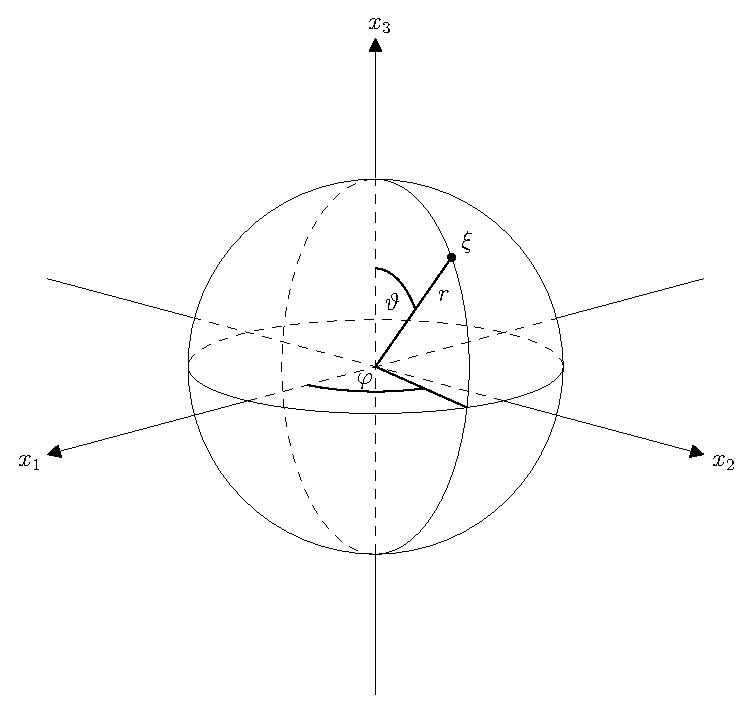
\includegraphics[height=12cm,width=12cm]{images/sphere}
  \caption{The spherical coordinate system in $\R^3$. Every point $\xi$ on a
  sphere with radius $r$ around the origin can be uniquely described by angles 
  $\vtheta$, $\vphi$ and the radius $r$. For $\vtheta = 0$ or
  $\vtheta = \pi$ the point $\xi$ coincides with the North or the South
  pole, respectively.}
  \label{sphere}
\end{figure}

\section{Legendre-type functions}
\label{Basics:LegendreTypeFunctions}
In this section we shortly define \emph{Legendre Polynomials}, \emph{associated Legendre functions} 
and \emph{associated Legendre polynomials} and collect some basic properties. These functions play 
a major role in Fourier analysis on the sphere and are key for the algorithms related to Fourier 
expansions developed in this text.

The Legendre polynomials $P_k : \interv{[}{-1}{1}{]} \rightarrow \R$, $k \in \N_{0}$ 
as classical orthogonal polynomials are given by their corresponding 
\emph{Rodrigues-formula}
\begin{equation}
  \nonumber
  \fun{P_k}{x} = \frac{1}{2^k k!} \frac{\dx^k}{\dx x^k} \paren{x^2-1}^k.
\end{equation}
The corresponding three-term recurrence relation is
\begin{equation}
  \nonumber
  \paren{k+1}\fun{P_{k+1}}{x} = \paren{2k+1}x\fun{P_{k}}{x} -
  k\fun{P_{k-1}}{x},\ k \in \N.
\end{equation}

Furthermore one defines the associated Legendre functions $P_k^n : \interv{[}{-1}{1}{]} \rightarrow \R$, 
$n \in \NZ$, $k=n,n+1,\ldots$ as 
\begin{equation}
  \nonumber
  \fun{P_k^n}{x} := \paren{\frac{\paren{k-n}!}{\paren{k+n}!}}^{1/2}
  \paren{1-x^2}^{n/2} \frac{\dx^n}{\dx x^n} \fun{P_k}{x}.
\end{equation}
For fixed $n$ the functions $\set{P_{k}^n}_{k=n,n+1,\ldots}$ form a complete set of orthogonal functions 
for $\Ln{2}{\interv{[}{-1}{1}{]}}$ with
$$ \frac{1}{2} \int_{-1}^{1} \fun{P_{k}^n}{x} \fun{P_{l}^n}{x} \dx x = \frac{1}{2k+1} \delta_{k,l}.$$
Furthermore, associated Legendre functions fulfill the recurrence relation
\begin{eqnarray*}
  & & \fun{P_{n-1}^n}{x} := 0,\qquad \fun{P_{n}^n}{x} = \frac{((2n)!)}{2^n n!}^{1/2} \paren{1-x^2}^{n/2},\\
  & & \fun{P_{k+1}^n}{x} = v_{k}^n x \fun{P_{k}^n}{x} + w_{k}^n \fun{P_{k-1}^n}{x} \quad (k = n,n+1,\ldots),
\end{eqnarray*}
where
$$ v_{k}^n := \frac{2k+1}{((k-n+1)(k+n+1))^{1/2}}\; ,\qquad w_{k}^n := - \frac{((k-n)(k+n))^{1/2}}{((k-n+1)(k+n+1))^{1/2}}\; .$$
A simple but at the same time very important idea is to define the associated Legendre functions also for 
$k < n$ by means of the three-term recurrence relation
$$ \fun{P_{k+1}^n}{x} = \paren{\alpha_{k}^n x \beta_{k}^n} \fun{P_{k}^n}{x} + \gamma_{k}^n \fun{P_{k-1}^n}{x} $$
with
\begin{eqnarray*}
  \alpha_{k}^n & := & \left\{
    \begin{array}{ll}
      (-1)^{k+1} & \text{for}\ k < n,\\
      v_{k}^n    & \text{otherwise},
    \end{array}\right.\\
  \beta_{k}^n & := & \left\{
    \begin{array}{lll}
      1 & \text{for}\ k < n,\\
      0 & \text{otherwise},
    \end{array}\right.\\
  \gamma_{k}^n & := & \left\{
    \begin{array}{lll}
      0       & \text{for}\ k \leq n,\\
      w_{k}^n & \text{otherwise.}
    \end{array}\right.\\
\end{eqnarray*}
For even $n$ one sets 
$$ \fun{P_{-1}^n}{x} := 0,\ \fun{P_{0}^n}{x} := \sqrt{\frac{(2n)!}{2^n n!}}$$
and for odd $n$
$$ \fun{P_{0}^n}{x} := \fun{P_{1}^n}{x} := \sqrt{\frac{(2n)!}{2^n n!}} \paren{1-x^2}^{1/2}$$
respectively. For $k >= n$ these functions coincide with the associated Legendre functions as defined above. 
As a matter of fact, $P_{k}^n$ is a polynomial of degree $k$ for even $n$ while $\paren{1-x^2}^{-1/2}P_{k}^n$
is a polynomial of degree $k-1$ for odd $n$.

Based on the recurrence coefficients from Equation \eqref{} and introducing a shift parameter $c \in \NZ$, one 
defines the associated Legendre polynomials $\fun{P_{k}^n}{\cdot,c}$ by
\begin{eqnarray*}
  & & \fun{P_{-1}^n}{x,c} := 0,\ \fun{P_{0}^n}{x,c} := 1,\\
  & & \fun{P_{k+1}^n}{x,c} = \paren{\alpha_{k+c}^n x + \beta_{k+c}^n} \fun{P_{k}^n}{x,c} + \gamma_{k+c}^n \fun{P_{k-1}^n}{x,c}
\end{eqnarray*}
By induction one verifies the relation between associated Legendre functions and polynomials in the following lemma.
\begin{lemma}
  Let the functions $P_{k}^n$ and $\fun{P_{k}^n}{\cdot,c}$ be given as in Equation \eqref{} and 
  Equation \eqref{} respectively. Then it holds
  $$ \fun{P_{c+k}^n}{x} = \fun{P_{k}^n}{x,c} \fun{P_{c}^n}{x} + \gamma_{c}^n \fun{P_{k-1}^n}{x,c+1} \fun{P_{c-1}^n}{x}. $$
\end{lemma}

\newpage

They can be characterized in ways similar
to those for Legendre polynomials, for instance by the
corresponding Rodrigues-formula or a differential equation. They
play an important role in the definition of spherical harmonics.
Note that for $k = 0$, the associated Legendre functions coincide with 
the Legendre polynomials.
Now let $k,m,n \in \N_0$, $k \le \min\encl{\{}{m,n}{\}}$. Then the associated
Legendre functions fulfill the orthogonality condition
\begin{equation}
\nonumber
  \int_{-1}^{1} \fun{P_{m}^{k}}{t} \fun{P_{n}^{k}}{t}\;dt =
  \frac{2}{2n+1}\delta_{m,n}.
\end{equation}



%Starting with the {\it{Legendre polynomials}}
% $$
% P_{k}(x):= \frac{1}{2^k k!} \frac{\dx^k}{\dx x^k} (x^2-1)^k\quad (x
% \in [-1,1]; k \in \N_{0})\; ,
% $$
% we define the {\it{associated Legendre functions}} $P_{k}^n \; (n \in
% \N_{0}; k = n,n+1, \ldots )$ as\\
% \begin{eqnarray}
% \label{assi}
% P_{k}^n(x):=\left(\frac{(k-n)!}{(k+n)!} \right)^{1/2} (1-x^2)^{n/2}
% \frac{\dx^n}{\dx x^n} P_{k}(x)\quad (x \in [-1,1])\; .
% \end{eqnarray}
% For any fixed $n \in \N_{0}$, the functions $P_{k}^n (k=n,n+1,
% \ldots )$ form a complete orthogonal system in $L^2[-1,1]$ with
% $$
% \frac{1}{2} \int\limits_{-1}^1 P_{k}^n (x) P_{l}^n (x) \dx x =
% \frac{1}{2k+1} \delta_{k,l}\quad (n \in \N_{0}; k,l=n,n+1, \ldots )\; .
% $$
% Moreover, the associated Legendre functions fulfill the three-term
% recurrence relation
% $$
% P_{n-1}^n (x):=0,\qquad P_{n}^n
%(x)= \frac{((2n)!)}{2^n n!}^{1/2} (1-x^2)^{n/2}\; ,
%$$
%\begin{equation}
%    P_{k+1}^n (x)=v_{k}^n x P_{k}^n (x) + w_{k}^n P_{k-1}^n
%    (x)\quad (k=n,n+1, \ldots )
%    \end{equation}
%    with
%    $$
%    v_{k}^n:= \frac{2k+1}{((k-n+1)(k+n+1))^{1/2}}\; ,\qquad
%    w_{k}^n:= - \frac{((k-n)(k+n))^{1/2}}{((k-n+1)(k+n+1))^{1/2}}\; .
%    $$
%    A simple but powerful idea in \cite{postta97} is to define the
%    functions $P_{k}^n$  also for $k < n$.
%    This was done as follows.
%    For even $n$ we start with $P_{-1}^n:=0$ and $P_{0}^n (x):=
%    \frac{\sqrt{(2n)!}}{2^n n!}$ and for odd $n$ let $P_{0}^n
%    (x):=P_{1}^n (x):= 
%    \frac{\sqrt{(2n)!}}{2^n n!} (1-x^2)^{1/2}$. We introduce the
%    functions $P_{k}^n$ by the three-term recurrence relation
%\begin{eqnarray}\label{drei}
%    P_{k+1}^n (x) := (\alpha_{k}^n x+ \beta_{k}^n) P_{k}^n (x) +
%    \gamma_{k}^n P_{k-1}^n (x)
%    \end{eqnarray}
%with
%    $$
%    \begin{array}{lllll}
%        \alpha_{k}^n := \left\{\begin{array}{lll}
%        (-1)^{k+1} &\ \mbox{for}\ k < n,\\
%        v_{k}^n &\ \mbox{otherwise},
%    \end{array}\right.\\[3ex]
%    \beta_{k}^n := \left\{\begin{array}{lll}
%        1 &\ \mbox{for}\ k < n,\\
%        0 &\ \mbox{otherwise},
%    \end{array}\right.\\[3ex]
%    \gamma_{k}^n := \left\{\begin{array}{lll}
%        0 &\ \mbox{for}\ k \leq n,\\
%        w_{k}^n &\ \mbox{otherwise.}
%    \end{array}\right.\\
%        \end{array}
%        $$
% It is a fact, that $P_{k}^n$ is a polynomial of degree $k$
% for even $n$ and that $(1-x^2)^{-1/2} P_{k}^n$ is a polynomial of degree
% $k-1$ for odd $n$. Furthermore, these functions coincide with
% (\ref{assi}) for $k\ge n$.
%The main reason for defining $P_k^n$ also for $k<n$ is that this
%modification allows a stable computation of the Legendre function transform.



\section{Spherical Harmonics}
\label{Basics:SphericalHarmonics}

For harmonic analysis in $\R^3$ the complex exponentials $e^{i \V{\omega}^{\transp} \cdot}$ 
($\V{\omega} \in \R^3$) provide the standard Fourier basis. With respect to the sphere one derives
from Laplace's equation restricted to the sphere solutions forming an orthonormal basis similar to
complex exponentials. We begin by noting some facts on 
orthogonal Legendre polynomials and the closely related associated
Legendre functions. Based on this
foundation, we describe the function space of spherical harmonics
and how it is related to spherical approximation.

Concerning the generating series of the Legendre polynomials
\begin{equation}
\label{LengendreFunctionsAndSphericalHarmonics.LegendrePolynomials.PowerSeries}
  \fun{\phi}{h} := \sum_{n = 0}^{\infty} \fun{P_n}{t} h^n,\ t \in
  \interv{[}{-1}{1}{]}
\end{equation}
which is absolutely and uniformly convergent for $h \in
\interv{(}{-1}{1}{)}$, it holds
\begin{equation}
  \label{LengendreFunctionsAndSphericalHarmonics.LegendrePolynomials.SeriesExpansion}
    \sum_{n = 0}^{\infty} \fun{P_n}{t} h^n = \frac{1}{\sqrt{1-2ht+h^2}}.
\end{equation}
This follows from the ordinary differential equation
\begin{equation}
\label{LengendreFunctionsAndSphericalHarmonics.LegendrePolynomials.SeriesExplicit}
  \paren{1+h^2-2ht}\fun{\phi'}{h} = \paren{t-h}\fun{\phi}{h}
\end{equation}
obtained by differentiation with respect to $h$ and comparing coefficients in line with Equation
\eqref{LengendreFunctionsAndSphericalHarmonics.LegendrePolynomials.PowerSeries}. Using the initial 
condition $\fun{\phi}{0}=1$ this yields the unique solution in Equation
\eqref{LengendreFunctionsAndSphericalHarmonics.LegendrePolynomials.SeriesExplicit}.
From this result, the following identity follows easily:
\begin{equation}
  \sum_{n=0}^{\infty} \paren{2n+1} \fun{P_n}{t} h^n =
  \frac{1-h^2}{\paren{1-2ht+h^2}^{3/2}}.
\end{equation}

When $h$ is restricted to $\interv{(}{0}{1}{)}$, the function
$G_h:\interv{[}{-1}{1}{]} \rightarrow \R$, with
\begin{equation}
\label{PoissonKernel}
  \fun{G_h}{t} := \frac{1-h^2}{\paren{1-2ht+h^2}^{3/2}},
\end{equation}
is called \emph{Poisson kernel}. We refer 
to Figure \ref{LengendreFunctionsAndSphericalHarmonics.LegendrePolynomials.Figure.PoissonKernel}
for a visual impression and take notice of the fact that the parameter $h$
allows for controlling the concentration of the function's energy around
$t = 1$.

\begin{figure}[htb]
  \centering
  \includegraphics[height=9cm,width=12cm]{images/poisson}
  \caption{The Poisson kernel for different values of $h$. The $x$-axis is scaled
  linearly
  with respect to $\vtheta$ while the argument for the function is $t=\cos\vtheta$. Since the cosine
  function is monotone in the interval $\interv{[}{0}{\pi}{]}$, this yields a bijective mapping to
  the interval $\interv{[}{-1}{1}{]}$, where $\vtheta = 0$ and $\vtheta = \pi$ correspond to
  $t=1$ and $t=-1$. This is the fashion, this function will be used in further
  investigations. It can be seen clearly that the energy more and more concentrates around
  $\vtheta = 0$ as $h$ gets closer to 1.}
  \label{LengendreFunctionsAndSphericalHarmonics.LegendrePolynomials.Figure.PoissonKernel}
\end{figure}


We now introduce the function space of spherical harmonics, a key to the treatment of spherical approximation problems.
From Laplace's differential equation $\Delta f = 0$ in $\R^3$, one obtains in spherical coordinates
\begin{equation}
  \label{SphericalHarmonics.LaplaceEquation.SphericalCoordinates}
  \Delta f = \frac{\partial^2 f}{\partial r^2} + \frac{2}{r}\frac{\partial f}{\partial
  r} + \frac{1}{r^2 \sin \vtheta}\frac{\partial}{\partial \vtheta}\paren{\sin \vtheta \cdot \frac{\partial f}{\partial
  \vtheta}} + \frac{1}{r^2 \sin \vtheta}\frac{\partial^2}{\partial \vphi^2} = 0.
\end{equation}
Using an ansatz based on separation of variables and taking into account that $r = 1$, one obtains the solutions
\begin{equation}
  \label{LegendreFunctionsAndSphericalHarmonics.SphericalHarmonics}
  \begin{split}
    Y_{n,k}: \interv{[}{0}{\pi}{]}\times\interv{[}{0}{2\pi}{)} \rightarrow
    \C,\\
    \fun{Y_{n,k}}{\vtheta,\vphi} := \sqrt{\frac{2n+1}{4\pi}} 
    \fun{P_{n}^{\abs{k}}}{\cos \vtheta} e^{ik\vphi},
  \end{split}
\end{equation}
where $n \in \N_{0},\ k = -n,-n+1,\dots,n$.
An important result states that the functions $Y_{n,k}$ are contained in $\fun{\text{Harm}_n}{\twosphere}$.
Due to the separability one proves easily
that they also fulfill the orthogonality condition with respect to the standard scalar product on $\twosphere$:
\begin{equation}
\label{LengendreFunctionsAndSphericalHarmonics.SphericalHarmonics.Orthogonality1}
\scalarproduct{Y_{n,j}}{Y_{m,k}}_{\twosphere} = \delta_{j,k} \delta_{n,m}\end{equation}
If we now define $\mathcal{H}_n$ to be
$\text{Harm}_n\paren{\twosphere}$, then
for every $n \in \N_0$, the set
\begin{equation}
  \nonumber
  \pset{Y_{n,k}}{|}{-n \le k \le n}
\end{equation}
forms an orthonormal basis of $\mathcal{H}_n$, since $\dim \mathcal{H}_n =
2n+1$. Moreover, the spaces $\mathcal{H}_n$ are orthogonal
to each other and the set 
$$\pset{Y_{n,k}}{|}{n = 0,1,\dots,N,\ k = -n,-n+1,\dots,n},\ N \in
\N_0$$ provides an orthonormal basis for the space
$\bigoplus_{n=0}^{N}\mathcal{H}_n$ called
the space of \emph{spherical harmonics} of degree $N$.

At first glance, the restriction to homogeneous and harmonic polynomials
might exclude various functions from being as well representable
as in $\fun{\Pi_n}{\twosphere}$. But as a matter of fact these
spaces are identical, i.e. 
\begin{equation}
  \nonumber
    \fun{\Pi_N}{\twosphere} = \bigoplus_{n=0}^{N}\mathcal{H}_n.
\end{equation}

We finally mention the well-known addition theorem of
spherical harmonics that relates basis functions of
$\mathcal{H}_n$ and Legendre-polynomials.
For every $\fun{L^2}{\twosphere}$ orthonormal basis
$\set{Y_{n,k}}_{k=-n}^{n}$ of $\mathcal{H}_n$, it holds
\begin{equation}
\label{AdditionTheorem}
  \sum_{k=-n}^{n} \fun{Y_{n,k}}{\V{\xi}}
  \overline{\fun{Y_{n,k}}{\V{\eta}}} =
  \frac{2n+1}{4\pi}\fun{P_n}{\scalarproduct{\V{\xi}}{\V{\eta}}_{\twosphere}}.
\end{equation}

